\documentclass{scrartcl}
\usepackage[utf8]{inputenc}
%\usepackage[T1]{fontenc}
\usepackage[a4paper, left=2.5cm, right=2.5cm, top=2.5cm, bottom=4cm]{geometry}
\usepackage[english]{babel}
\usepackage{amsmath, amsthm, amssymb, amstext}
\usepackage{listings}
\usepackage{color}
\usepackage{graphicx}
\usepackage{xparse}
\usepackage{fancyhdr}
\usepackage{algorithmicx}
\usepackage{algpseudocode}
\usepackage{algorithm}
\usepackage{parskip}
\usepackage[table]{xcolor}
\usepackage{tabularx}
\usepackage{enumerate}
\usepackage{enumitem}
%\usepackage{minted}
\usepackage {tikz}
\usetikzlibrary{positioning}

\pagestyle{fancy}


\rhead{{\newcommand\and\\\getauthors}}
\author{Felix Bühler\\2973410 \and Clemens Lieb\\3130838 \and Steffen Wonner\\2862123 \and Fabian Bühler\\2953320}
\lhead{\textbf\gettitle}
\title{\gettitle}
\chead{\getsubtitle}
\subtitle{\getsubtitle}

\addtolength{\headheight}{2\baselineskip}
\renewcommand{\headrulewidth}{0pt}

\newcommand{\gettitle}{Distributed systems I\\Winter Term 2019/20}
\newcommand{\getsubtitle}{G2T1 – Assignment 4 (theoretical part)}
\newcommand{\getauthors}{Felix Bühler \and Clemens Lieb \and Steffen Wonner \and Fabian Bühler}
\setlength{\headheight}{53pt}

\begin{document}
\maketitle

\section*{1 - Global State}
\subsection*{a)}
\subsection*{b)}
\subsection*{c)}
\subsection*{d)}

\section*{2 - Transaction Processing}
\subsection*{a)}
The conflicting operation pairs are: 
\[\{(w_1[u], w_3[u]), (r_1[y], w_2[y]), (r_3[y], w_2[y]), (r_2[x], w_3[x])\}\]

\subsection*{b)}

\begin{figure}[ht!]
\begin{tikzpicture}
    \node[draw, circle] at (0, 0)    (T1) {\(T_1\)};
    \node[draw, circle] at (5, 0)    (T2) {\(T_2\)};
    \node[draw, circle] at (2.5,2.5) (T3) {\(T_3\)};

    \draw[->]
        (T1) edge node[above,sloped] {\(w_1[y] \to r_2[y]\)} (T2)
        (T2) edge node[above,sloped] {\(w_2[z] \to w_3[z]\)} (T3)
        (T3) edge node[above,sloped] {\(w_3[y] \to r_1[y]\)} (T1);
\end{tikzpicture}
\caption{Serialization Graph for History \(H_1\)}
\label{fig:sg_h1}
\end{figure}

It's clear that the serialization graph shown in Figure \ref{fig:sg_h1} contains a cycle, as such \(H_1\) is not serializable.\\~\\

\begin{figure}[ht!]
\begin{tikzpicture}
    \node[draw, circle] at (0, 0)    (T1) {\(T_1\)};
    \node[draw, circle] at (5, 0)    (T2) {\(T_2\)};
    \node[draw, circle] at (2.5,2.5) (T3) {\(T_3\)};

    \draw[->]
        (T2) edge node[above,sloped] {\(r_2[y] \to w_1[y]\)} (T1)
        (T3) edge node[above,sloped] {\(r_3[x] \to w_1[x]\)} (T1)
        (T3) edge node[above,sloped] {\parbox[c]{2.5cm}{\(r_3[x] \to w_2[x] \\ w_3[u] \to w_2[u]\)}} (T2);
\end{tikzpicture}
\caption{Serialization Graph for History \(H_2\)}
\label{fig:sg_h2}
\end{figure}

The serialization graph shown in Figure \ref{fig:sg_h2} does not contain a cycle, which would imply that \(H_2\) is serializable.\\
Unfortunately \(H_2\) is not a correct history as it does not specify the order or the conflicting operations \(w_1[x], w_2[x]\).



\section*{3 - Two-Phase Locking}

\end{document}
